\chapter{Test di performance}

% ======================================================
%a
% 4.1 - METHODOLOGY
%
% ======================================================
\section{Ambiente e metodologia}
I test sono stati eseguiti su un Apple M2 con 8 core, 4 ad alte prestazioni (\emph{performance core}) e 4 a basso consumo (\emph{efficiency core}), con Java 21.

Ogni misura comprende $M = 100$ passi, senza GUI, partendo dagli stessi corpi iniziali.

Come indice di prestazione si usa lo \emph{speedup}, ovvero il rapporto tra il tempo sequenziale e quello concorrente:
\[
  S = \frac{T_{seq}}{T_{par}}
\]

% ======================================================
%
% 4.2 - SEQUENTIAL COMPARISON
%
% ======================================================
\section{Confronto con la versione sequenziale}
In \cref{tab:confronto} sono riportati i tempi al variare del numero di corpi $N$, con 8 thread.

\begin{table}[H]
  \centering
  \begin{tabular}{rrrrrr}
    \toprule
    $N$ & Sequenziale & Thread & Executor & $S$ thread & $S$ executor \\
    \midrule
    500    & 37 ms    & 23 ms    & 33 ms    & 1,61 & 1,11 \\
    1\,000 & 176 ms   & 60 ms    & 95 ms    & 2,91 & 1,85 \\
    2\,000 & 641 ms   & 240 ms   & 261 ms   & 2,67 & 2,45 \\
    5\,000 & 3\,997 ms & 1\,231 ms & 1\,185 ms & 3,25 & 3,37 \\
    \bottomrule
  \end{tabular}
  \caption{Tempo di 100 passi al variare del numero di corpi, con 8 thread.}
  \label{tab:confronto}
\end{table}

Entrambe le versioni concorrenti sono più veloci di quella sequenziale, e il vantaggio cresce con $N$: il calcolo cresce come $N^2$, mentre il costo della sincronizzazione resta costante.
Con pochi corpi l'Executor è più lento, perché i suoi $2N$ task per passo svolgono poco lavoro ciascuno; con $N = 5\,000$ le due versioni si equivalgono.

% ======================================================
%
% 4.3 - SCALABILITY
%
% ======================================================
\clearpage
\section{Scalabilità rispetto al numero di core}
Con $N = 5\,000$ corpi e da 1 a 8 thread si ottengono i tempi di \cref{tab:scalabilita} e lo speedup di \cref{fig:speedup} ($T_{seq} = 3\,997$ ms).

\begin{table}[H]
  \centering
  \begin{tabular}{rrrrr}
    \toprule
    N. thread & Thread & Executor & $S$ thread & $S$ executor \\
    \midrule
    1 & 4\,039 ms & 4\,773 ms & 0,99 & 0,84 \\
    2 & 2\,239 ms & 2\,693 ms & 1,78 & 1,48 \\
    3 & 1\,714 ms & 1\,903 ms & 2,33 & 2,10 \\
    4 & 1\,593 ms & 1\,681 ms & 2,51 & 2,38 \\
    5 & 1\,578 ms & 1\,536 ms & 2,53 & 2,60 \\
    6 & 1\,461 ms & 1\,462 ms & 2,74 & 2,73 \\
    7 & 1\,294 ms & 1\,500 ms & 3,09 & 2,67 \\
    8 & 1\,393 ms & 1\,367 ms & 2,87 & 2,92 \\
    \bottomrule
  \end{tabular}
  \caption{Tempo di 100 passi con $N = 5\,000$ corpi, al variare del numero di thread.}
  \label{tab:scalabilita}
\end{table}

\begin{figure}[tb]
  \centering
  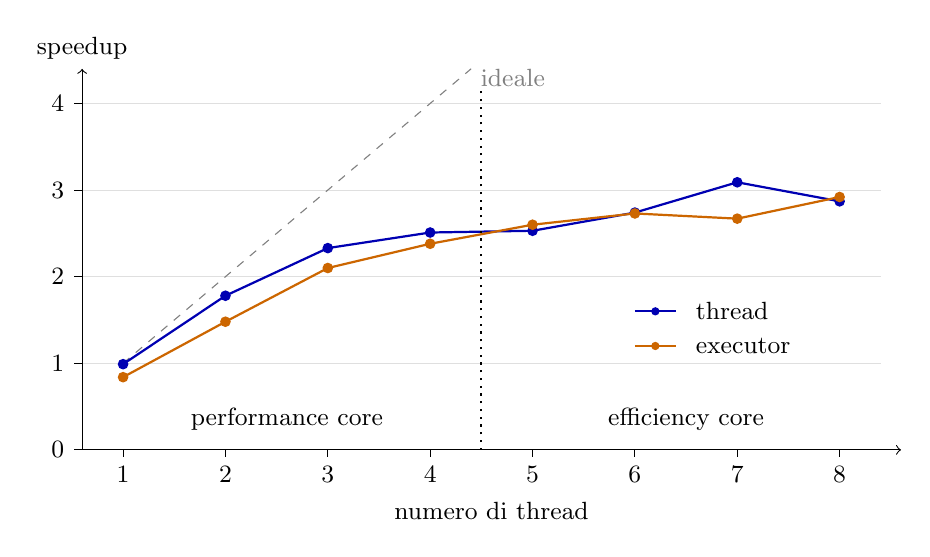
\begin{tikzpicture}[x=1.3cm, y=1.1cm]
    % grid and axes
    \foreach \y in {1,2,3,4}
      \draw[gray!25] (0.6, \y) -- (8.4, \y);
    \draw[->] (0.6, 0) -- (8.6, 0);
    \node[font=\small] at (4.6, -0.7) {numero di thread};
    \draw[->] (0.6, 0) -- (0.6, 4.4) node[above, font=\small] {speedup};
    \foreach \x in {1,...,8}
      \draw (\x, 0) -- (\x, -0.08) node[below, font=\small] {\x};
    \foreach \y in {0,...,4}
      \draw (0.6, \y) -- (0.52, \y) node[left, font=\small] {\y};
    % ideal speedup
    \draw[dashed, gray] (1, 1) -- (4.4, 4.4);
    \node[gray, font=\small, anchor=west] at (4.4, 4.3) {ideale};
    % thread version
    \draw[thick, blue!70!black] plot[mark=*, mark size=1.5pt] coordinates
      {(1,0.99) (2,1.78) (3,2.33) (4,2.51) (5,2.53) (6,2.74) (7,3.09) (8,2.87)};
    % executor version
    \draw[thick, orange!80!black] plot[mark=*, mark size=1.5pt] coordinates
      {(1,0.84) (2,1.48) (3,2.10) (4,2.38) (5,2.60) (6,2.73) (7,2.67) (8,2.92)};
    % separation between performance and efficiency cores
    \draw[dotted, thick] (4.5, 0) -- (4.5, 4.2);
    \node[font=\small] at (2.6, 0.35) {performance core};
    \node[font=\small] at (6.5, 0.35) {efficiency core};
    % legend
    \begin{scope}[shift={(6.0, 1.6)}, font=\small]
      \draw[thick, blue!70!black] (0, 0) -- (0.4, 0); \fill[blue!70!black] (0.2, 0) circle (1.5pt);
      \node[anchor=west] at (0.5, 0) {thread};
      \draw[thick, orange!80!black] (0, -0.4) -- (0.4, -0.4); \fill[orange!80!black] (0.2, -0.4) circle (1.5pt);
      \node[anchor=west] at (0.5, -0.4) {executor};
    \end{scope}
  \end{tikzpicture}
  \caption{Speedup rispetto alla versione sequenziale, con $N = 5\,000$ corpi.}
  \label{fig:speedup}
\end{figure}

Con un thread la versione multithread eguaglia quella sequenziale, quindi la barriera costa poco, mentre l'Executor è più lento del 16\% per la gestione dei task.
Lo speedup cresce rapidamente fino a 4 thread, poi molto più lentamente, fino a circa 3 con 8 thread.

% ======================================================
%
% 4.4 - DISCUSSION
%
% ======================================================
\section{Discussione dei risultati}
Entrambe le versioni concorrenti migliorano le prestazioni, con uno speedup massimo di circa $3{,}3$ su 8 core.
Lo speedup resta lontano da quello ideale perché solo 4 core sono ad alte prestazioni: oltre il quarto, i thread finiscono sui core più lenti e, a ogni barriera, tutti attendono il più lento.
L'Executor ne risente meno, perché assegna i task dinamicamente e i core più veloci ne eseguono di più.
Con 6--8 thread le misure variano di più, a causa dello scheduling del sistema operativo.
